\thesolution{Ribalta}
L'approccio in generale pi� efficiente per ribaltare la lista consiste nel modificare la configurazione di tutti i puntatori contenuti nella struttura, senza pertanto effettuare spostamenti fisici di elementi. Di seguito si forniscono due soluzioni, la prima basata su un metodo iterativo, la seconda su uno ricorsivo.

\begin{figure}
  \begin{center}
    \begin{minipage}{.8\textwidth}
      \subfigure[Lista originale]{
        \centering
        \label{fig:Originale}
        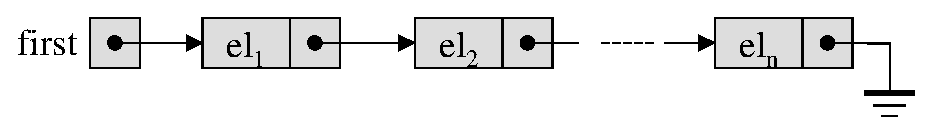
\includegraphics[width=.9\textwidth]{Esercizi/Ribalta/Originale.eps}
      }%
    \end{minipage}
    \hfill
    \begin{minipage}{.6\textwidth}
      \subfigure[Prima dell'i-esima iterazione]{
        \centering
        \label{fig:PrimaDelWhile}
        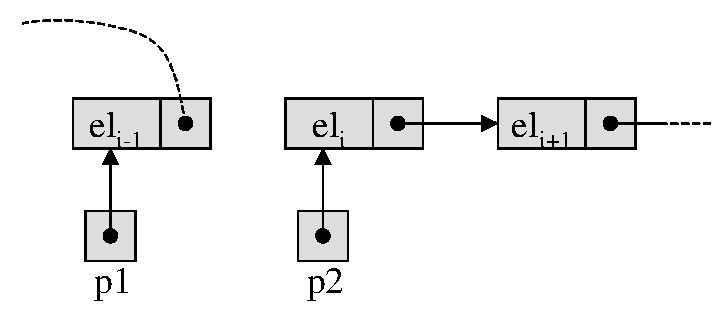
\includegraphics[width=.9\textwidth]{Esercizi/Ribalta/PrimaDelWhile.eps}
      }%
    \end{minipage}
    \hfill
    \begin{minipage}{.6\textwidth}
      \subfigure[Dopo l'i-esima iterazione]{
        \centering
        \label{fig:DopoIlWhile}
        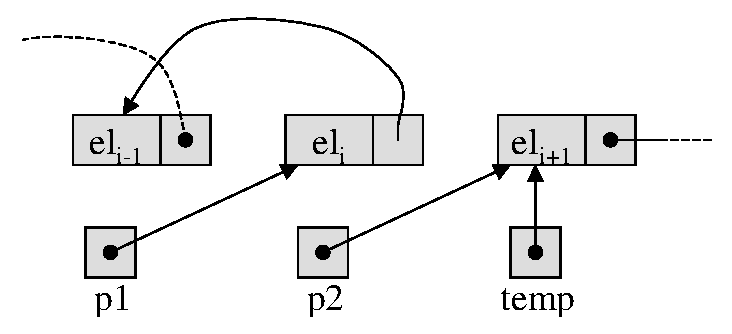
\includegraphics[width=.9\textwidth]{Esercizi/Ribalta/DopoIlWhile.eps}
    }
    \end{minipage}
    \hfill
    \begin{minipage}{.8\textwidth}
      \subfigure[Lista ribaltata]{
        \centering
        \label{fig:Ribaltata}
        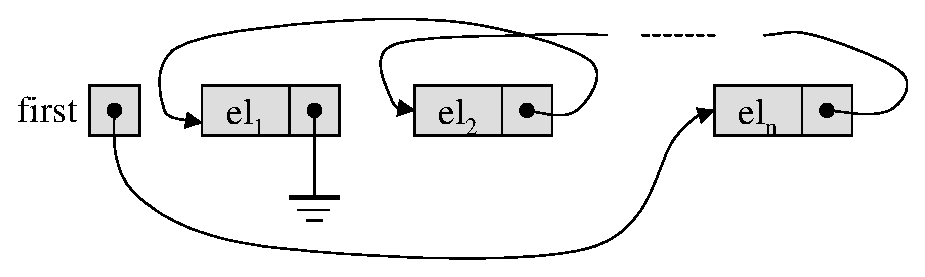
\includegraphics[width=.9\textwidth]{Esercizi/Ribalta/Ribaltata.eps}
    }
    \end{minipage}
  \end{center}
  \caption{Il processo logico di ribaltamento di una lista}
  \label{fig:Ribaltamento}
\end{figure}

\subsubsection*{Approccio iterativo}
Si consideri la \figurename~\ref{fig:Originale}, in cui � riportata la lista di partenza. Per ottenerne il ribaltamento � sufficiente che il campo \cod{succ} del primo elemento (che punta ad $el_2$) passi a puntare a 0, che il campo \cod{succ} del secondo elemento (che punta ad $el_3$) passi a puntare al primo, che il campo \cod{succ} del terzo elemento (che punta ad $el_4$) passi a puntare al secondo\ldots\ e cos� via. Infine, il puntatore \cod{first} (che punta ad $el_1$) dovr� puntare all'elemento $el_n$. Questo procedimento pu� essere svolto servendosi di due puntatori che iniziano a scorrere la lista nell'unica direzione concessa, puntando di volta in volta a due elementi consecutivi e spostandosi in avanti di un elemento alla volta. Ad ogni passo dell'iterazione lo scambio pu� essere effettuato servendosi di un terzo puntatore temporaneo (vedi Figure~\ref{fig:PrimaDelWhile} e~\ref{fig:DopoIlWhile}). Lo stato finale della lista al termine dell'iterazione � riportato in \figurename~\ref{fig:Ribaltata}.

%\begin{figure}
%  \begin{center}
%    \begin{minipage}{.8\textwidth}
%      \subfigure[prima dell'i-esima iterazione]{
%        \centering
%        \label{fig:PrimaDelWhile}
%        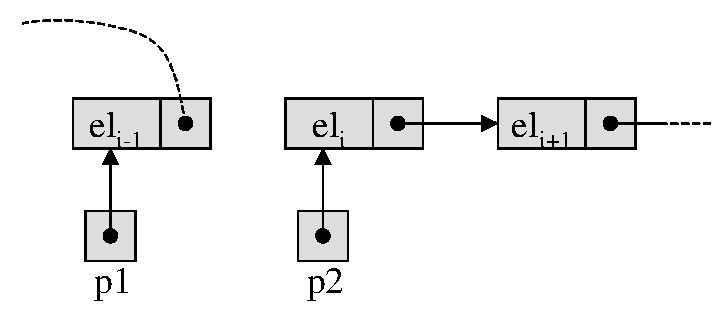
\includegraphics[width=.9\textwidth]{Esercizi/Ribalta/PrimaDelWhile.eps}
%      }%
%    \end{minipage}
%    \hfill
%    \begin{minipage}{.8\textwidth}
%      \subfigure[dopo l'i-esima iterazione]{
%        \centering
%        \label{fig:DopoIlWhile}
%        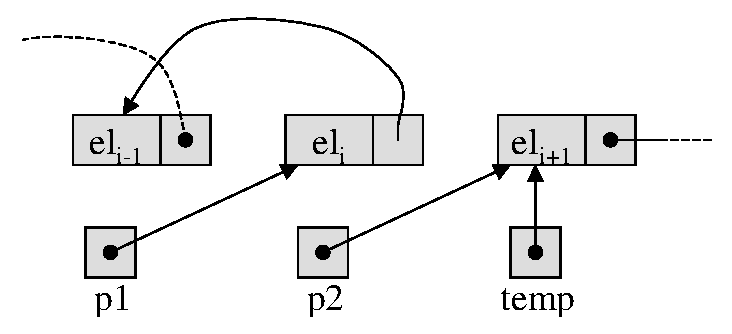
\includegraphics[width=.9\textwidth]{Esercizi/Ribalta/DopoIlWhile.eps}
%    }
%    \end{minipage}
%  \end{center}
%  \caption{Effetto dell'i-esima iterazione}
%  \label{fig:iesimaiterazione}
%\end{figure}

\bigskip
\inputprogram{Esercizi/Ribalta/Ribalta_iterativo.cpp}

\subsubsection*{Approccio ricorsivo}
Il ribaltamento della lista pu� essere approcciato come un problema ricorsivo. Infatti, avendo una lista, la sua versione ribaltata si ottiene isolando il primo elemento, ribaltando la restante parte della lista, e posponendo a questa l'elemento isolato. Il problema del ribaltamento di una lista si riconduce dunque al ribaltamento di una seconda lista costituita da un elemento in meno. Di questo passo ci si trover� a ribaltare una lista costituita da un unico elemento, la cui versione ribaltata � uguale a s� stessa. Durante il processo di ribaltamento bisogna anche prestare attenzione a redirigere correttamente la testa della (sotto)lista di volta in volta considerata. A questo proposito, il metodo ricorsivo \cod{\_Ribalta()} riceve in ingresso il puntatore alla testa della lista da ribaltare e restituisce la testa della lista ribaltata.

\bigskip
\inputprogram{Esercizi/Ribalta/Ribalta_ricorsivo.cpp}